\section{Typchecker mit Typinferenz}

Im letzten Kapitel haben wir gesehen, wie der Benutzer ein Prinzip mit
Hilfe der PrincipleWriter User Language aufschreiben kann, und wie die
Mozart/Oz-Repr\"asentation der abstrakten Syntax, die das Parsermodul
aus der PWUL generiert, aussieht.

Da Typfehler vom Parser nicht erkannt werden, wird das Typcheckermodul
gebraucht.  Aber das Typcheckermodul kann noch mehr, es kann fast alle
Typen inferieren, so dass der Benutzer praktisch gar keine Typen mehr
annotieren muss, was das Schreiben von Prinzipien noch weiter
vereinfacht. Warum Typannotationen \"uberhaupt notwendig sind, werden
wir sp\"ater bei der \"Ubersetzung der Formeln in Constraints in
Mozart/Oz sehen.

Der Typchecker arbeitet direkt mit der Mozart/Oz-Repr\"asentation der
abstrakten Syntax, die wie gesehen ein Record ist, der den Parsebaum
repr\"asentiert. Der Parsebaum wird vom Typchecker um Typannotationen
erweitert. Um die Arbeitsweise zu veranschaulichen verwenden wir
Inferenzregeln. Dabei wurde kein vollst\"andiges Typsystem entwickelt,
die Regeln dienen nur zum einfachen Aufschreiben der verschiedenen
F\"alle. Als Beispiel die Regel f\"ur eine Variable mit Typannotation:
\footnote{Auch wenn der Typchecker nicht mit der konkreten Syntax
  arbeitet, sondern mit der abstrakten, verwenden wir wegen der
  besseren Lesbarkeit die PrincipleWriter User Language Syntax in den
  Regeln.}

\InferNoName{\Gamma \vdash \mathtt{x::type}}
      {\Gamma \cup \{x \mapsto type\} \vdash \mathtt{x::type}}
      {x \mapsto T \in \Gamma \Rightarrow T=\mathit{type}}
     
Sie besagt, dass wenn wir einen Kontext $\Gamma$ haben, und eine Variable
{\tt x} mit Typannotation {\tt type} finden, wir $x \mapsto \mathit{type}$
in den Kontext aufnehmen, sofern die Variable {\tt x} nicht schon im
Kontext mit einem anderen Typ ist. Die Formel wird nicht ver\"andert.
Der Kontext mappt Variablen auf Typen. Die Seitenbedingungen der
Regeln werden nicht nur f\"ur die Typinferenz, sondern vor allem auch
f\"ur das Typchecking gebraucht. Wertet die Formel in der
Seitenbendingung zu {\tt false} aus, wird eine Fehlermeldung
ausgegeben.

\subsection{Arbeitsweise des Typcheckers}

Um die Typen \"uberpr\"ufen bzw.\ inferieren zu k\"onnen, steigt der
Typchecker von der Wurzel des Parsebaums abw\"arts zu den Bl\"attern
und merkt sich auf dem Weg die Variablen, die noch zu inferieren sind,
und die Variablen-Typ Paare, die er schon erkannt hat, bzw.\ die
annotiert sind. An einem Blatt angekommen, bewegt er sich wieder
zur\"uck in Richtung der Wurzel, und vereinigt an jedem Knoten die
Kontexte, die an diesem Knoten zusammenkommen auf dem Weg zur Wurzel.
Lassen sich die Kontexte nicht vereinigen, z.B.\ wegen eines
Typeclashes, wird mit einer Fehlermeldung abgebrochen.

Bevor wir uns das Typchecking mit Typinferenz f\"ur einige
ausgew\"ahlte Regeln und deren Implementierungen anschauen werden ein
paar Hilfsfunktionen beschrieben.

\subsubsection{Die Funktion {\tt Type}}

Das Typchecking wird angesto{\ss}en durch die Funktion {\tt Type}, die
als Argument den Record, den der Parser gebaut hat, nimmt, und einen
vollst\"andig getypten Record zur\"uckliefert.  Betrachten wir uns den
Anfang des Parsebaums, der mit den folgenden drei Regeln gebildet
wird: \Equsl{rcl}{1.0}{%
  \UlS&::=&\UlDefType* \UlDefPrinciple+\\
  \UlDefType&::=&\Ulp{deftype}\ \UlConstant\ \UlType\\
  \UlDefPrinciple&::=&\Ulp{defprinciple}\ \UlConstant\ \Ulp{\{}\
  \UlDims\ \UlConstraints\ \Ulp{\}}}{eq:irgendwas} {\tt Type} erstellt
eine Liste mit den Constraints aus dem Parsebaum. Das sind die
Formeln, die gecheckt werden sollen. F\"ur jede Formel ruft {\tt Type}
die Hauptfunktion {\tt DecideStrategy} auf, die das Typchecking
\"ubernimmt.  Da durch das Abschneiden des oberen Teils des Baumes
Informationen \"uber vom Prinzipienschreiber definierte Typbenennungen
verloren gehen, erstellt {\tt Type} vorher einen Record mit dieser
Information.  Daf\"ur wird die Funktion {\tt CollectDefTypes}
verwendet. Dieser Record wird an {\tt DecideStrategy} \"ubergeben,
ebenso wie ein leerer Kontext.

\subsubsection{Die Funktion {\tt CollectDefTypes}}\label{collectdeftypes}

Die mit {\tt deftype} vom Grammatikschreiber definierten
Typbenennungen werden von der Funktion {\tt CollectDefTypes} aus dem
ihr \"ubergebenen kompletten Parsebaum extrahiert, und in einem Record
gespeichert, das Typnamen auf Typen abbildet.

\subsubsection{Die Funktion {\tt UnionContext}}

% \begin{figure}
% \begin{verbatim}
% fun {UnionContext Context1 Context2}
%    As1 = {Arity Context1}
%    As2 = {Arity Context2}
%    As21 = {Filter As2
%            fun {$ A2} {Not {Member A2 As1}} end}
%    As = {Append As1 As21}
%    ATTups =
%    {Map As
%     fun {$ A}
%        T1 = {CondSelect Context1 A undef}
%        T2 = {CondSelect Context2 A undef}
%        T =
%        if T1==T2 then
%           T1
%        else
%           T11 = if T1==undef then _ else T1 end
%           T21 = if T2==undef then _ else T2 end
%        in
%           try
%              T11 = T21
%           catch E then
%              {Inspector.inspect E}
%           end
%           T11
%        end
%     in
%        A#T
%     end}
%    ATRec = {List.toRecord o ATTups}
% in
%    ATRec
% end
% \end{verbatim}
% \caption{Quellcode der Funktion {\tt UnionContext}}
% \label{UnionContextCode}
% \end{figure}
Der Kontext des Typcheckers besteht aus einem Record, das Variable-Typ
Paare enth\"alt. Die Funktion {\tt UnionContext} versucht zwei
Kontexte zu vereinigen. Dabei wird \"uberpr\"uft, dass es keine zwei
Variablen mit unterschiedlichen Typen gibt, was einen Typeclash
ausl\"osen w\"urde.

% In Abbildung~\ref{UnionContextCode} ist der Mozart/Oz-Quellcode der
% Funktion zu sehen. Zuerst wird eine List mit allen Namen der beiden
% Kontexte erstellt (Zeilen 2-6), wobei durch Zeilen 4-5 ein doppeltes
% Auftreten von Namen verhindert wird.

% In den Zeilen 8-28 wird dann jedem Namen aus der Liste der
% entsprechende Typ angef\"ugt, und damit der neue Kontext
% gebildet. Daf\"ur wird f\"ur jeden Namen zuerst der Typ aus den zwei
% Ursprungskontexten bestimmt (Zeilen 10 und 11). Wenn die beiden Typen
% gleich sind, kann der Typ einfach an den Namen angef\"ugt werden
% (Zeilen 13 und 14). Sollten die Typen nicht gleich sein, muss
% \"uberpr\"uft werden, ob einer der beiden Typen noch nicht definiert
% ist. Falls dies der Fall ist, werden in den Zeilen 16 und 17 die
% Variable {\tt T11} bzw.\ {\tt T12} auf den noch nicht definierten Wert
% {\tt \_} gesetzt. Falls der Typ nicht undefiniert ist, werden den
% Variablen die entsprechenden Typen zugewiesen. In dem darauf folgenden
% try-catch Block wird versucht, eine L\"osung f\"ur den Constraint {\tt
% T11 = T12} zu finden, was nur gelingt, wenn eine der beiden Variablen
% noch nicht definiert ist. Falls keine L\"osung gefunden werden kann
% hat man einen Typeclash gefunden. Liegt kein Typeclash vor, wird der
% Typ, den die Variablen jetzt beide enthalten an den Namen angeh\"angt.

\subsection{Die Implementation des eigentlichen Typcheckings}

Nachdem wir die Hilfsfunktionen vorgestellt haben, kommen wir jetzt zum
Kern des Typinferenzmoduls, der von den Funktionen {\tt
  DecideStrategy} und {\tt TypeNonQuantifier} gebildet wird.  {\tt
  DecideStrategy} \"ubernimmt das Typchecking und die Typinferenz
f\"ur die Quantoren. Sie stellt auch den Startpunkt dar, da sie von
{\tt Type} aufgerufen wird. Ist der oberste Knoten im Baum kein
Quantor, \"ubergibt sie den Baum an {\tt TypeNonQuantifier}, ansonsten
versucht sie den Quantor zu typen, indem sie sich mit der Formel
hinter dem Quantor rekursiv aufruft.  {\tt TypeNonQuantifier} ruft
nicht sich selbst rekursiv wieder auf, sondern ruft {\tt
  DecideStrategy} auf. Die Teilung in die zwei Funktionen hat den
Grund die Lesbarkeit des Quellcodes zu steigern.

Beide Funktionen bekommen als Argumente den Record {\tt
  ConstantATypeTreeRec} der die Abbildung von Typnamen auf Typen
enth\"alt (Siehe Funktion CollectDefTypes, Seite
\pageref{collectdeftypes}), die mit {\tt deftype} vom
Grammatikschreiber definiert wurden. Als zweites Argument einen
Kontext und als drittes eine Formel, die getypt, bzw.\ \"uberpr\"uft
werden soll.

Beide Funktionen haben als R\"uckgabewert einen Record der Form:
\begin{verbatim}
o(operation:TypedForm
  con:NewContext)
\end{verbatim}
wobei {\tt TypedForm} die Eingabeformel ist, die um Typannotationen
erg\"anzt wurde, und deren Typen \"uberpr\"uft wurden. {\tt
  NewContext} ist der Kontext, nachdem die Eingabeformel bearbeitet
wurde.

Die gesamte Implementierung der beiden Funktionen wollen wir uns nicht
anschauen, sondern lediglich ein paar ausgesuchte Beispiele.

\subsubsection{Die Funktion {\tt DecideStrategy}}

\begin{figure}
\Infer{\begin{array}{l}
        \Gamma \vdash \mathtt{exists~ X::type:Form} \\
        \Gamma \cup \{X \mapsto \mathit{type}\} \vdash \mathtt{Form}
       \end{array}}
      {\Gamma \vdash \mathtt{exists~ X::type:Form}}
      {(\mathit{type} \in \mathit{Dom})}
      {$\exists$, getypt}
\Infer{\begin{array}{l}
        \Gamma \vdash \mathtt{exists~ X:Form} \\
        \Gamma \cup \{X \mapsto \mathit{type}\} \vdash \mathtt{Form}
       \end{array}}
      {\Gamma \vdash \mathtt{exists~ X::type:Form}}
      {(\mathit{type} \in \mathit{Dom})}
      {$\exists$, ungetypt, inferrierbar}
\Infer{\begin{array}{l}
        \Gamma \vdash \mathtt{exists~ X:Form} \\
        \Gamma \vdash \mathtt{Form}
       \end{array}}
      {\mathtt{Error: Could not infer Type of X}}
      {\begin{array}{l}
     (\mathit{con} \mapsto T \notin \Gamma) \vee\\
     (T=\_)
     \end{array}}
   {$\exists$, ungetypt, nicht inferrierbar}
\caption{Die Regeln f\"ur das Typchecking des $\exists$ Quantors}
\label{existsrules}
\end{figure}

\begin{figure}
% \begin{verbatim}
% fun {DecideStrategy ConstantATypeTreeRec Context Form}
%    FirstOp = Form.sem
% in
%    case FirstOp
%    of exists(ConstantTree DomTree FormTree) then
%      VarName = {Helpers.constantTree2A ConstantTree}
%      Dom = {Helpers.tree2T DomTree ConstantATypeTreeRec}
%      NewContext = {UnionContext Context o(VarName:Dom)}
%      NewValues = {DecideStrategy 
%                   ConstantATypeTreeRec NewContext FormTree}
%    in
%       o(operation:exists(ConstantTree DomTree NewValues.operation)
%         con:NewValues.con)
%    [] exists(ConstantTree FormTree) then
%       VarName = {Helpers.constantTree2A ConstantTree}
%    in
%       if {HasFeature Context VarName} then
%          raise 'ERROR: Variable already defined'#VarName end
%       else
%          NewContext = {UnionContext Context o(VarName:undef)}
%          NewValues = {DecideStrategy 
%                       ConstantATypeTreeRec NewContext FormTree}
%       in
%          case NewValues.con.VarName
%          of undef then
%             raise 'ERROR: Variable has no type'#VarName end
%          else
%             o(operation:exists(ConstantTree 
%                                NewValues.con.VarName 
%                                NewValues.operation)
%               con:NewValues.con)
%          end
%       end
%    else
%       {TypeNonQuantifier ConstantATypeTreeRec Context Form}
%    end
% end
% \end{verbatim}
\begin{center}
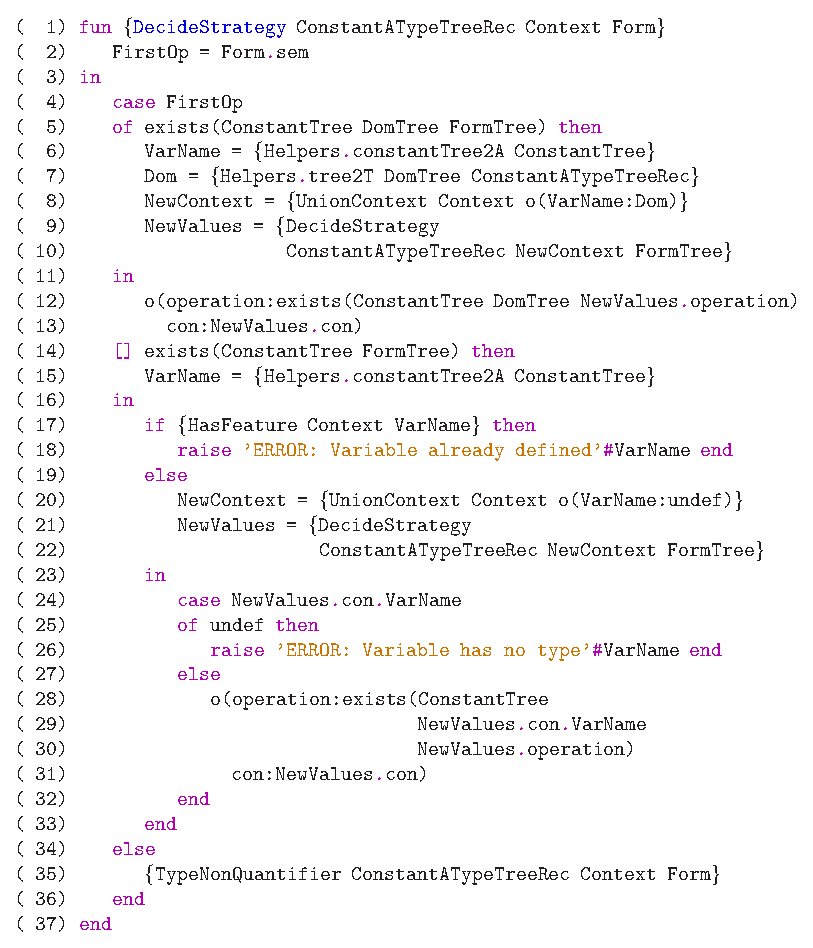
\includegraphics[scale=1.0]{eps/decide_n}
\end{center}
\caption{Quellcode der Funktion {\tt DecideStrategy}}
\label{DecideStrategyCode}
\end{figure}

Bevor wir die Implementierung von {\tt DecideStrategy} am Beispiel des
$\exists$-Quantors erkl\"aren, werden wir uns die Regeln f\"ur den
Quantor anschauen. Die Regeln und die Implementierung der anderen
Quantoren funktioniert analog.

F\"ur das Typchecking und die Typinferenz von Quantoren werden drei
F\"alle unterschieden. In Abbildung~\ref{existsrules} sind die drei
Regeln zu sehen. Die erste Regel behandelt den Fall, dass schon eine
Typannotation an der Variablen {\tt X}, \"uber die quantifiziert wird,
existiert. In diesem Fall wird versucht, die Typen der Formel {\tt
  Form} zu checken, bzw.\ zu inferieren, wobei $X \mapsto
\mathit{type}$ in den Context \"ubernommen wird. K\"onnen die Typen
von {\tt Form} inferiert und \"uberpr\"uft werden, wird $X \mapsto
\mathit{type}$ wieder aus dem Kontext entfernt, da diese Variable im
Baum nur innerhalb von {\tt Form} vorkommen darf. Sollte die Variable
an einer anderen Stelle vorkommen, muss sie an einen anderen
Quantor gebunden sein.

Die zweite Regel steht f\"ur den Fall, dass keine Typannotation an der
Variablen {\tt X} vorliegt, der Typ aber aus der Formel {\tt Form}
inferiert werden kann. Wenn dies der Fall ist enth\"alt der Kontext,
nachdem {\tt Form} bearbeitet wurde, einen Eintrag f\"ur die Variable
{\tt X}. Dieser Eintrag wird aus dem Kontext entfernt, nachdem der Typ
dann annotiert wurde.

Die dritte Regel beschreibt, dass keine Typannotation vorliegt, und
der Typ von {\tt X} auch nicht aus der Formel {\tt Form} inferiert
werden konnte. Dann bricht der Typchecker mit einer Fehlermeldung ab.

Schauen wir uns die Implementierung von {\tt DecideStrategy} an, die
in Abbildung~\ref{DecideStrategyCode} zu sehen ist. In Zeile 2 wird
die zu untersuchende Formel aus der abstrakten Syntax extrahiert.
Danach folgt eine Fallunterscheidung, wo durch Pattern-Matching
entweder der $\exists$-Quantor mit Typannotation gefunden wird (Zeilen
5--13), oder ohne Typannotation (Zeilen 14--33) Die F\"alle f\"ur die
anderen Quantoren sind nicht aufgef\"uhrt. Wird kein Quantor gefunden,
wird der Baum und der Kontext an {\tt TypeNonQuantifier} weitergegeben
(Zeile 35).

Im ersten Fall wird in Zeile 6 der Name der Variable aus dem Parsebaum
extrahiert. Zeile 7 extrahiert den Typ aus dem Unterbaum {\tt
  DomTree}.  Danach wird das Paar aus dem Variablennamen und dem Typ
in den Kontext aufgenommen (Zeile 8). In Zeile 9 folgt der rekursive
Aufruf f\"ur die Formel nach dem Quantor {\tt FormTree} mit dem neuen
Kontext.

In den Zeilen 12 und 13 wird dann der R\"uckgaberecord gebaut, wobei
der Unterbaum {\tt FormTree} durch den bearbeiteten Baum aus dem
rekursiven Aufruf ersetzt wird. Als Kontext wird der Kontext aus dem
rekursiven Aufruf zur\"uckgegeben, aus dem das in Zeile 8
hinzugef\"ugte Paar wieder entfernt wurde.

Beim zweiten Fall wird auch erst der Variablenname bestimmt (Zeile
15). Danach wird \"uberpr\"uft ob die Variable schon im Kontext ist,
und falls ja eine Fehlermeldung ausgegeben. Ist die Variable noch
nicht im Kontext, wird sie diesem mit unbestimmtem Typ ({\tt undef})
hinzugef\"ugt (Zeile 20). In Zeile 21 folgt dann die Rekursion mit
neuem Kontext f\"ur die Formel {\tt FormTree}. In den Zeilen 24 und 25
wird dann gepr\"uft, ob der rekursive Aufruf den Typ der Variablen
inferieren konnte. Falls nicht, wird entsprechend der Regel 3 eine
Fehlermeldung ausgegeben. Konnte der Typ ermittelt werden, wird der
Ausgaberecord gebaut, indem dem Baum die Typannotation hinzugef\"ugt
wird (Zeile 29), und {\tt FormTree} durch den bearbeiteten Baum aus
dem rekursiven Aufruf ersetzt wird. Dies entspricht Regel 2.

\subsubsection{Die Funktion {\tt TypeNonQuantifier}}

% \begin{figure}
% \StarInfer{\Gamma \vdash \mathtt{Expr}_1 ~ \mathtt{in ~ Expr}_2 \mathtt{::set(label(D))}}
% {\begin{array}{l}
% \Gamma \cup \{Expr_1 \mapsto label(D), Expr_2 \mapsto set(label(D)) \\
% \vdash \mathtt{Expr}_1 \mathtt{::label(D) ~ in ~ Expr}_2 \mathtt{::set(label(D))}
% \end{array}
% }
% {\begin{array}{r l}
%         \text{*} & Expr_{1-2} \mapsto T \notin \Gamma \vee\\
%          & (Expr_1 \mapsto T_1 \in \Gamma \Rightarrow T_1= (label(D) \wedge \_) \vee\\
%          & Expr_2 \mapsto T_2 \in \Gamma \Rightarrow T_2=(set(label(D)) \wedge \_))
%          \end{array}
% }
% {Element, teilweise annotiert, inferrierbar}

% \StarInfer{\Gamma \vdash \mathtt{Expr}_1 \mathtt{::label(D) ~ in ~ Expr}_2}
% {\begin{array}{l}
% \Gamma \cup \{Expr_1 \mapsto label(D), Expr_2 \mapsto set(label(D)) \\
% \vdash \mathtt{Expr}_1 \mathtt{::label(D) ~ in ~ Expr}_2 \mathtt{::set(label(D))}
% \end{array}
% }
% {\begin{array}{r l}
%         \text{*} & Expr_{1-2} \mapsto T \notin \Gamma \vee\\
%          & (Expr_1 \mapsto T_1 \in \Gamma \Rightarrow T_1= (label(D) \wedge \_) \vee\\
%          & Expr_2 \mapsto T_2 \in \Gamma \Rightarrow T_2=(set(label(D)) \wedge \_))
%          \end{array}
% }
% {Element, teilweise annotiert, inferrierbar}

% \StarInfer{\Gamma \cup \{Expr_1 \mapsto label(D) \} \vdash \mathtt{Expr}_1 \mathtt{~ in ~ Expr}_2}
% {\begin{array}{l}
% \Gamma \cup \{Expr_1 \mapsto label(D), Expr_2 \mapsto set(label(D)) \\
% \vdash \mathtt{Expr}_1 \mathtt{::label(D) ~ in ~ Expr}_2 \mathtt{::set(label(D))}
% \end{array}
% }
% {\begin{array}{r l}
%         \text{*} & Expr_{2} \mapsto T \notin \Gamma \vee\\
%          & Expr_2 \mapsto T_2 \in \Gamma \Rightarrow T_2=(set(label(D)) \wedge \_))
%          \end{array}
% }
% {Element, inferrierbar}

% \StarInfer{\Gamma \cup \{Expr_2 \mapsto set(label(D)) \} \vdash \mathtt{Expr}_1 \mathtt{~ in ~ Expr}_2}
% {\begin{array}{l}
% \Gamma \cup \{Expr_1 \mapsto label(D), Expr_2 \mapsto set(label(D)) \\
% \vdash \mathtt{Expr}_1 \mathtt{::label(D) ~ in ~ Expr}_2 \mathtt{::set(label(D))}
% \end{array}
% }
% {\begin{array}{r l}
%         \text{*} & Expr_{1} \mapsto T \notin \Gamma \vee\\
%          & Expr_1 \mapsto T_1 \in \Gamma \Rightarrow T_1=(label(D) \wedge \_))
%          \end{array}
% }
% {Element, inferrierbar}
% \caption{Die Regeln f\"ur das Typchecking von $\in$}
% \label{inrules}
% \end{figure}

% \begin{figure}
% \begin{verbatim}
% [] 'in'(ExprTree1 ExprTree2) then
%    DoneExprTree1 = {DecideStrategy 
%                     ConstantATypeTreeRec Context ExprTree1}
%    DoneExprTree2 = {DecideStrategy 
%                     ConstantATypeTreeRec Context ExprTree2}
%    NewContext1 = {UnionContext Context DoneExprTree1.con}
%    NewContext2 = {UnionContext Context DoneExprTree2.con}
%    NewContext = {UnionContext NewContext1 NewContext2}
%    TypeExprTree1 = if {HasFeature DoneExprTree1.operation anno} then
%                       DoneExprTree1.operation.anno.2
%                    else
%                       notype1
%                    end
%   TypeExprTree2 = if {HasFeature DoneExprTree2.operation anno} then
%                       DoneExprTree1.operation.anno.2
%                   else
%                      notype1
%                   end
% in
%    case TypeExprTree2 of
%       set(Type) then
%       if TypeExprTree1 == notype1 then
%           o(operation:'in'(anno(DoneExprTree1.operation Type) 
%                            DoneExprTree2.operation) 
%             con:NewContext)
%       else
%          raise "Couldn't determine type" end
%       end
%    [] notype1 then
%       if TypeExprTree1 \= notype1 then
%          o(operation:'in'(DoneExprTree1.operation 
%                           anno(DoneExprTree2.operation 
%                                set(TypeExprTree1))) 
%            con:NewContext)
%       else
%          raise "Couldn't determine type" end
%       end
%    else
%       if TypeExprTree2.set == TypeExprTree1 then
%           o(operation:'in'(DoneExprTree1.operation 
%                            DoneExprTree2.operation) 
%             con:NewContext)
%       else
%          raise "Typeclash" end
%       end
%    end
% \end{verbatim}
% \caption{Quellcode f\"ur {\tt in}}
% \label{incode}
% \end{figure}
% \begin{figure}
% \StarInfer{\Gamma \vdash \mathtt{edge(Con}_1 ~ \mathtt{Con}_2 ~ \mathtt{Con}_3 ~
% \mathtt{Con}_4)}
%       {\begin{array}{l}
%         \Gamma \cup \{Con_1 \mapsto node, Con_2 \mapsto node, Con_3
%         \mapsto dim, Con_4 \mapsto label(Con_4)\}\\
%         \vdash \mathtt{edge(Con}_1  \mathtt{::node ~ Con}_2 
%         \mathtt{::node ~ Con}_3 \mathtt{::dim~
%         Con}_4\mathtt{::label(Con}_4 \mathtt{))}
%        \end{array}}
%        {\begin{array}{r l}
%         \text{*} & Con_{1-4} \mapsto T \notin \Gamma \vee\\
%          & (Con_1 \mapsto T_1 \in \Gamma \Rightarrow T_1= (node \wedge \_) \vee\\
%          & Con_2 \mapsto T_2 \in \Gamma \Rightarrow T_2=(node \wedge \_)\vee\\
%          & Con_3 \mapsto T_3 \in \Gamma \Rightarrow T_3=(dim \wedge \_)\vee\\
%          & Con_4 \mapsto T_4 \in \Gamma \Rightarrow T_4=(label(Con_4)) \wedge \_)\\
 
%         \end{array}}
%       {$v_1 \overset{l}{\rightarrow}_d v_2$}

% \caption{Die Regel f\"ur eine gelabelte Kante}
% \label{edgerule}
% \end{figure}
% \begin{figure}
% \begin{verbatim}
%       [] ledge(TermTree1 TermTree2 TermTree3 TermTree4) then
% 	 %% %
% 	 ConstantAI1 = {Helpers.termTree2AI TermTree1}
% 	 ConstantS1 = {V2S ConstantAI1}
% 	 NewContext1 =
% 	 if {Char.isAlpha ConstantS1.1} andthen
% 	    {Char.isUpper ConstantS1.1} andthen
% 	    {All ConstantS1
% 	     fun {$ Ch}
% 		{Char.isAlpha Ch} orelse {Char.isDigit Ch}
% 	     end}
% 	 then
% 	    {UnionContext Context o(ConstantAI1:node)}
% 	 else
% 	    Context
% 	 end
% 	 ConstantAI2 = {Helpers.termTree2AI TermTree2}
% 	 ConstantS2 = {V2S ConstantAI2}
% 	 NewContext2 =
% 	 if {Char.isAlpha ConstantS2.1} andthen
% 	    {Char.isUpper ConstantS2.1} andthen
% 	    {All ConstantS2
% 	     fun {$ Ch}
% 		{Char.isAlpha Ch} orelse {Char.isDigit Ch}
% 	     end}
% 	 then
% 	    {UnionContext NewContext1 o(ConstantAI2:node)}
% 	 else
% 	    NewContext1
% 	 end
% 	 ConstantAI3 = {Helpers.termTree2AI TermTree3}
% 	 ConstantS3 = {V2S ConstantAI3}
% 	 NewContext3 =
% 	 if {Char.isAlpha ConstantS3.1} andthen
% 	    {Char.isUpper ConstantS3.1} andthen
% 	    {All ConstantS3
% 	     fun {$ Ch}
% 		{Char.isAlpha Ch} orelse {Char.isDigit Ch}
% 	     end}
% 	 then
% 	    T = {Helpers.tree2T TermTree4}
% 	 in
% 	    {UnionContext NewContext2 o(ConstantAI3:label(T))}
% 	 else
% 	    NewContext2
% 	 end
%       in
% 	 o(operation:ledge(TermTree1 TermTree2 TermTree3 TermTree4)
% 	   con:NewContext3)
% \end{verbatim}
% \caption{Quellcode f\"ur {\tt ledge}}
% \label{edgecode}
% \end{figure}
\begin{figure}
\Infer{\Gamma \vdash \mathtt{edge(v1 ~ v2 ~ d)}}
      {\Gamma \vdash \mathtt{edge(v1 ~ v2 ~ d)}}
       {}
      {$v_1 \rightarrow_d v_2~~v_1,v_2$ sind Konstanten}
\Infer{\Gamma \vdash \mathtt{edge(v1 ~ v2 ~ d)}}
      {\begin{array}{l}
        \Gamma \cup \{\mathit{v1} \mapsto \mathit{node}, \mathit{v2} \mapsto \mathit{node}, d
        \mapsto \mathit{dim}\}\\
        \vdash \mathtt{edge(v1 ~ v2 ~ d)}
       \end{array}}
       {\begin{array}{l}
         (\mathit{v1} \mapsto T_1 \in \Gamma \Rightarrow T_1=\mathit{node}) \wedge \\
         (\mathit{v2} \mapsto T_2 \in \Gamma \Rightarrow T_2=\mathit{node}) \wedge \\
         (d \mapsto T_3 \in \Gamma \Rightarrow T_3=\mathit{dim})
       \end{array}}
      {$v_1 \rightarrow_d v_2~~v_1,v_2 ,d$ sind Variablen}
\caption{Regel f\"ur das Typchecking einer ungelabelten Kante}
\label{edgerules}
\end{figure}

\begin{figure}
% \begin{verbatim}
% [] edge(TermTree1 TermTree2 TermTree3) then
%    ConstantAI1 = {Helpers.termTree2AI TermTree1}
%    ConstantS1 = {V2S ConstantAI1}
%    NewContext1 =
%    if {Char.isAlpha ConstantS1.1} andthen
%       {Char.isUpper ConstantS1.1} andthen
%       {All ConstantS1
%        fun {$ Ch}
%           {Char.isAlpha Ch} orelse {Char.isDigit Ch}
%        end}
%    then
%       {UnionContext Context o(ConstantAI1:node)}
%    else
%       Context
%    end
%       ConstantAI2 = {Helpers.termTree2AI TermTree2}
%       ConstantS2 = {V2S ConstantAI2}
%       NewContext2 =
%       if {Char.isAlpha ConstantS2.1} andthen
%          {Char.isUpper ConstantS2.1} andthen
%          {All ConstantS2
%           fun {$ Ch}
%              {Char.isAlpha Ch} orelse {Char.isDigit Ch}
%           end}
%       then
%          {UnionContext NewContext1 o(ConstantAI2:node)}
%       else
%          NewContext1
%       end
%       ConstantAI3 = {Helpers.termTree2AI TermTree3}
%       ConstantS3 = {V2S ConstantAI3}
%       NewContext3 =
%       if {Char.isAlpha ConstantS3.1} andthen
%          {Char.isUpper ConstantS3.1} andthen
%          {All Constant S3
%           fun {$ Ch}
%              {Char.isAlpha Ch} orelse {Char.isDigit Ch}
%           end}
%       then
%          {UnionContext NewContext2 o(ConstantAI3:dim)}
%       else 
%          NewContext2
%       end
%    in
%       o(operation:edge(TermTree1 TermTree2 TermTree3)
%         con:NewContext3)
% \end{verbatim}
\begin{center}
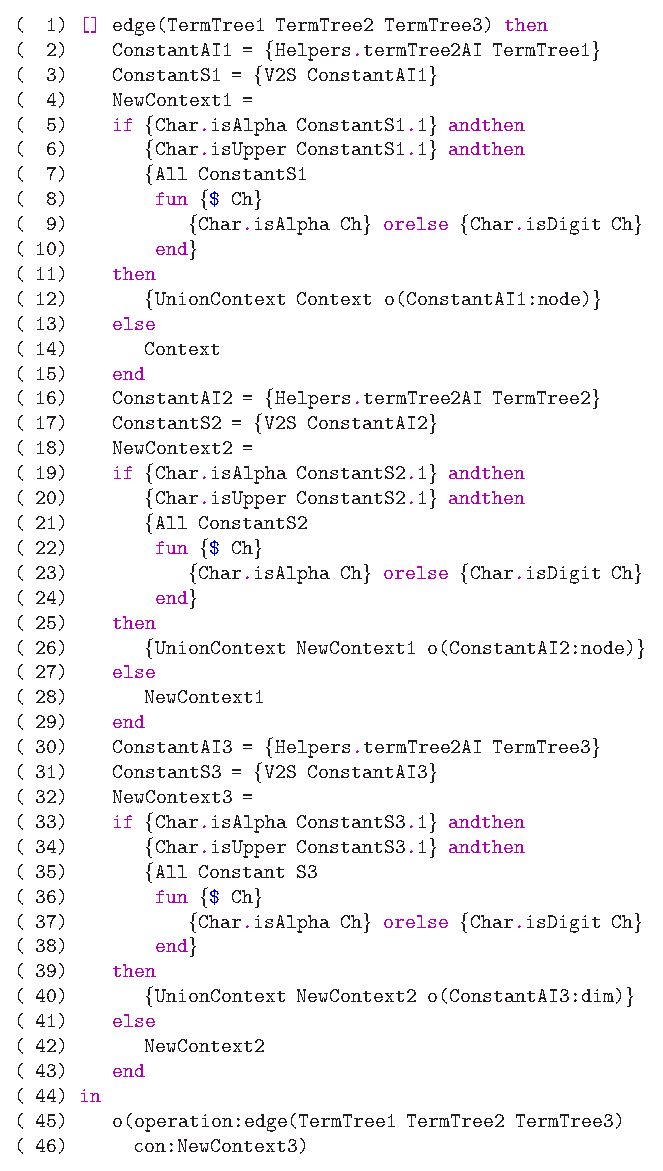
\includegraphics[scale=1.0]{eps/edge_n}
\end{center}
\caption{Quellcode des Typcheckings f\"ur eine ungelabelte Kante aus
  der Funktion {\tt TypeNonQuantifier}}
\label{edgecode}
\end{figure}

Um die Funktion {\tt TypeNonQuantifier} kennen zu lernen, schauen wir
uns zuerst an, wie die Kanten von ihr behandelt werden.
Abbildung~\ref{edgerules} zeigt zwei Regeln f\"ur ungelabelte Kanten.
Die Typen f\"ur {\tt v1}, {\tt v2} und {\tt d} m\"ussen nicht
ermittelt werden, da Kanten nur zwischen Knoten vorkommen d\"urfen.
{\tt d} ist immer vom Typ {\tt dim}. Es muss nur noch \"uberpr\"uft
werden, ob {\tt v1},{\tt v2} und {\tt d} Konstanten oder Variablen
sind. Ist {\tt v1},{\tt v2} oder {\tt d} eine Variable, wird sie in
den Kontext mit Typ {\tt node}, bzw.\ {\tt dim} \"ubernommen, falls das
zu keinem Typeclash f\"uhrt.  Der Parsebaum wird nicht ver\"andert, da
auch f\"ur die Evaluierung hier keine Typannotationen n\"otig sind.

Abbildung~\ref{edgecode} zeigt den Teil der Funktion {\tt
  TypeNonQuantifier}, der ungelabelte Kanten bearbeitet. Aus den drei
Unterb\"aumen, die die Knoten und die Dimension repr\"asentieren,
werden jeweils die Namen extrahiert, und dann gepr\"uft ob es
Variablen oder Konstanten sind. Falls es Konstanten sind werden sie in
den Kontext aufgenommen. Der neue Kontext wird dann zusammen mit dem
unver\"anderten Parsebaum zur\"uckgegeben. Da in dem rekursiven Ablauf
bei jeder Regel die ver\"anderten Kontexte nach oben gereicht werden,
k\"onnen die Variablen der Quantoren annotiert werden, falls der Typ
inferiert werden konnte.

\subsection{Beispiel CSD-Prinzip}

Zur Veranschaulichung werfen wir einen kurzen Blick auf das
CSD-Prinzip. Ohne die Typinferenz m\"usste das Prinzip so geschrieben
werden:
% \begin{verbatim}
% defprinciple "principle.csdPW" {
%   dims {D}
%   constraints {

%     forall V::node: forall V1::node:
%       edge(V V1 n D) =>
%         forall V2::node: 
%           forall V3::node: dom(V2 V D) & edge(V2 V3 n D) => V3<V1
%   }
% }
% \end{verbatim}
\begin{center}
\includegraphics[scale=1.0]{eps/csdvorher}
\end{center}

Mit der Typinferenz m\"ussen gar keine Typen mehr annotiert werden,
was das Schreiben von Prinzipien stark erleichtert:
% \begin{verbatim}
% defprinciple "principle.csdPW" {
%   dims {D}
%   constraints {

%     forall V: forall V1:
%       edge(V V1 n D) =>
%         forall V2: 
%           forall V3: dom(V2 V D) & edge(V2 V3 n D) => V3<V1
%   }
% }
% \end{verbatim}
\begin{center}
\includegraphics[scale=1.0]{eps/csdnachher}
\end{center}
